\documentclass[11pt, a4paper, oneside, openany]{book}

% Input and output encoding
\usepackage[utf8]{inputenc}
\usepackage[T1]{fontenc}

\usepackage[english]{babel}

\usepackage[dvipsnames]{xcolor}
\usepackage{lmodern}
\usepackage{enumitem}
\usepackage{todonotes}
\usepackage{setspace}
\usepackage{graphicx}
\usepackage{amssymb,amsmath}
\usepackage{mathtools}
\usepackage{float}
\usepackage[pass]{geometry}
\usepackage{ifdraft}

% Source code listings
\usepackage{minted}
\usemintedstyle{friendly}
\newminted{hs}{autogobble,linenos}

\usepackage[ unicode=true,
    plainpages=false,
    pdfpagelabels,
    draft=false,
    colorlinks=true,
    hyperfootnotes=false,
    linkcolor={Sepia},
    citecolor={PineGreen},
    urlcolor={MidnightBlue},
]{hyperref}

\hypersetup{
    pdfauthor={Kirill Vorozhtsov},
    pdftitle={Musikk},
    pdfsubject={Bachelor's Thesis}
}

\usepackage[
    backend=biber,
    style=numeric,
    sortlocale=en_GB,
    maxnames=100
]{biblatex}
\addbibresource{bibliography.bib}
\setlength{\tabcolsep}{6pt}

% % % % % % % % % % % % % % % % % % % % % % % % % % % % % % % % % % % % % % % %

\begin{document}
    \frontmatter
    \pagestyle{empty}

\begin{center}
{\Large \textsc{Masarykova univerzita}}

{\large \textsc{fakulta informatiky}}
    \vskip4em
    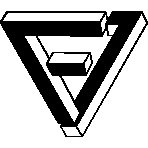
\includegraphics[width=4cm, height=4cm, draft=false] {logo_fi}
    \vskip4em
        {\begin{spacing}{1}
             \Huge \textbf{Musikk. A music streaming platform with social features.} % XXX: Title
    \end{spacing}}
    \vskip2em
        {\Large \textsc{Bachelor's Thesis}} % XXX: Type
    \vskip2em
        {\LARGE \textbf{Kirill Vorozhtsov}} % XXX: Author
    \vfill
    {\hfill\large Brno, 2025} % XXX: Year
\end{center}

\cleardoublepage
\restoregeometry

    \section*{Prohlášení} Prohlašuji, že tato práce je mým původním autorským dílem,
které jsem vypracoval samostatně. Všechny zdroje, prameny a literaturu, které
jsem při vypracování používal nebo z~nich čerpal, v~práci řádně cituji
s~uvedením úplného odkazu na příslušný zdroj.

\vfill\noindent
\textbf{Vedoucí práce:} Tvá babka   % XXX
\cleardoublepage

\section*{Poděkování} % XXX
\cleardoublepage

\section*{Shrnutí} % XXX

\subsection*{Klíčová slova} % XXX


    \setcounter{tocdepth}{2}
    \tableofcontents
    \pagestyle{plain}

    \mainmatter
    \chapter{Introduction}\label{chap:intro}


In recent years, with rapid development of the Internet,
music has become an even more integral part of everyday life.\cite{music_role_life}
It has never been easier to experience and share music — we have come
a long way from sharing vinyl records to simply sending a link to a streaming platform of choice.
Consequently, music has integrated even deeper into social interactions between people,
helping them bond and share strong emotional experiences.\cite{music_role_life}
\\
One of the direct impacts of this trend is the fast emergence of numerous music-related platforms.
While some focus on traditional music journalism or statistics, others offer unlimited access to audio content.
Naturally, people have started to discover and engage with music that resonates with them more frequently.\cite{music_role_life}
\\
Despite this, it is surprising that features which facilitate social interactions are not widely implemented in the
existing platforms, as will be shown in \nameref{chap:platforms}
\\
The goal of this thesis is to design a music-centric platform that embraces
collaboration and social interaction around music.
\\
This work is divided into the following \textbf{six} chapters:

\begin{enumerate}
    \item \textbf{\nameref{chap:survey}}
    Presents the outcomes of a survey illustrating how people consume music,
    how prevalent it is in social interactions, and why this thesis is relevant.

    \item \textbf{\nameref{chap:platforms}}
    Compares existing streaming solutions, music-related services
    and explores relevant non-musical platforms.

    \item \textbf{\nameref{chap:specs}}
    Outlines the functional and non-functional criteria for the application.

    \item \textbf{\nameref{ch:planning}}
    Describes the choices of technologies that are used by the application.

    \item \textbf{\nameref{chap:implementation}}
    Explains the development process and implementation details.

    \item \textbf{\nameref{chap:conclusion}}
    Summarizes the results and discusses possible improvements.
\end{enumerate}
    \chapter{Music Consumption Survey}\label{chap:survey}


\section{Background and objectives}
In order to better rationalize the topic of the thesis and show that a music streaming platform
is relevant as a service, a brief survey was conducted. It examines the
individual content‐consumption preferences, listening and discovery habits, platform usage patterns, and
social behaviours.


\section{Methods}
The platform chosen for the questionnaire was `Google Forms`\cite{googleforms}, as it provides a simple interface for
survey creation, allows for easy sharing of the form, and supports exporting the results to a spreadsheet.\\

The questionnaire itself consists of 15 questions.
Most of them are multi-choice and closed-ended with some having a possibility for a custom answer.\\

As for the respondents - 119 people had participated, with most being from Russian-speaking countries;
the majority was in the 18 to 30 age group, with the exact distribution shown in *fig.*

\subsection{Engagement}
Firstly, it was necessary to determine the actual frequency of engagement with audio content -- if the numbers were low,
it would indicate that a dedicated platform with advanced features might not be relevant for most users.
However, over 50\% of respondents reported listening to more than 500 songs per month *fig.*,
and nearly 80\% stated that they listen to music daily *fig.*.
This clearly shows that music is essential to many people, and the following logical step would be to discover
how the audio content is mostly accessed. \\

\subsection{Listening Methods}
As can be clearly seen in *fig* the percentage of streaming platforms usage across all ages is nearing 100\% with
slightly higher numbers in lower age groups. Although, downloaded files and physical media have their presence, especially for
people aged 30-60, it is usually only an auxiliary option next to the streaming solutions.
\\
Regarding the platforms themselves - Spotify has taken the first place in terms of popularity, proving the
global statistics\cite{spotifypopularity}. However, Yandex Music being in the second place deserves an explanation.
As mentioned previously, most of the respondents are from Russian-speaking countries, Russia specifically.
With a lot of western companies leaving its market in 2022, music streaming services included, most of the users has
moved to locally available services - Yandex Music, VK Music, Zvuk, and others.
Another notable point is the absence of other popular region-specific platforms, such as Amazon Music for the US market,
QQ music for the Chinese market or JioSaavn for the Indian one,
as all of the respondents were based in the european part of the world.
The full statistics are shown in *fig*.\\
Being established that streaming services are indeed widely-used and are in demand, the next important step would be
to analyze the regularity of music-centered social interactions.

\subsection{Social Interactions}
The results of Question 10 indicate that nearly all respondents (99.2\%) reported listening to music with
others, primarily in offline settings such as gatherings or car rides.
Online co-listening methods, while less common, were also mentioned by a quarter of respondents,
showing that digital solutions for shared listening are used, though not as prevalently as in-person scenarios.
\\
Question 11 investigates how often these interactions occur —
the results show that a significant portion of respondents engage in shared listening regularly.
Around 60\% reported doing so at least a few times per month,
with a smaller group indicating almost daily interactions.
This reinforces the idea that music consumption is a common social activity.
\\
The next question is phrased as following - "How often do you/your friends share/discuss music?".
While the previous question focused on real-time in-person collective listening,
this one highlights more intentional and in-depth musical interactions — such as sharing songs,
recommending music, or discussing it. Music in that case is not just the background but the main subject of engagement.
The same trend as before can be observed in the responses: a majority of participants reported engaging in these exchanges regularly.
Over 70\% indicated that they share music at least several times a month, with many doing so weekly or more often.
This further emphasizes the active social role of music.
\\
Question 13 — “How does that happen?” — provides an insight into the specific means of sharing.
Many respondents stated that they typically send links from streaming platforms through external messaging apps.
While this shows a clear demand for sharing music, it also reveals a gap: these interactions are fragmented across platforms.
Hence, enabling such exchanges directly within the streaming app could offer a smoother, more uniform experience.
\\
Responses to the question \textit{“Would you say that you know a lot of people with similar music taste?”} were mixed,
with a near-even split between those who do and do not.
This suggests that while some users already have a social circle with similar music taste, many do not.
Interestingly, when asked
\textit{“Would you like to connect with others who share your musical taste, or influence those around you to explore and appreciate the music you enjoy?”},
the majority answered positively.
This indicates a clear interest in expanding musical connections and supports the idea that social discovery
features could be useful within a streaming platform.
This is further supported by the responses to Question 15, where over 60\% of participants stated they would use
additional social features, if available on current streaming platforms.


\section{Results}
Overall, the results show that music is a vital part of many peoples' lives
and that streaming services are the main way people listen to it.
Music consumption is frequent, social, and often includes sharing and discovering new tracks.
Yet, current platforms only partly support these interactions.
Therefore, the idea of a music streaming service with integrated social features could be relevant,
addressing real user needs.


\begin{table}[ht]
    \label{tab:where_listen}
\end{table}
    \chapter{Existing Platforms}
In order to better understand what instruments people use when interacting with music,
it’s useful to examine existing solutions.


% TODO: add pictures for examples without links?


\section{Streaming Services}
% TODO: ref to survey table
As it can be seen from the table~\ref{tab:where_listen} and further confirmed by
the recent study of the International Federation of the Phonographic Industry\cite{music_stats_2024},
nowadays, the most prevalent way of music consumption
and discovery is the streaming services. There are many platforms available,
but only those that are both popular and feature unique elements will be considered.
The descriptions, rather than offering general information, will focus on the social aspects of each platform.

\begin{itemize}
    \item \textbf{Spotify} \\
    One of the most prominent social features on Spotify is the 'Spotify Jam'\cite{spotify_jam}.
    It lets people create a collective song queue which is then synchronized among all connected users.
    Moreover, volume, the order of songs and other aspects of the playback can be controlled individually.
    Another notable tool is the 'Blend' playlists\cite{spotify_recs}. These are playlists created automatically
    between two people, which contain songs matching audio preferences of both users.
    Lastly, 'Friend Activity'\cite{spotify_friend_activ}, which shows what the people you follow are currently listening to,
    and 'Listening Parties' that are live chats with a limited capacity,
    which can be joined for a short time when new music is being released\cite{spotify_party_1,spotify_party_2}.

    \item \textbf{VK Music} \\
    As was mentioned previously, this a music service integrated into the VK social network.
    Consequently, it is possible to send songs and playlists via private messages and add audio materials to
    posts in groups. VK Music also supports algorithmic playlists based on the groups that a user follows.
    It analyzes audio files posted in the specific groups and puts similar songs in those playlists.

    \item \textbf{SoundCloud} \\
    SoundCloud is one of the few platforms which lets its users leave comments
    and reactions on songs and playlists\cite{sc_comments,sc_reactions}.
    In addition, each user has a feed, consisting of his personal uploads and
    reposts of other's content\cite{sc_reposts}, which is visible when visiting his profile.

    \item \textbf{Bandcamp} \\
    Every Bandcamp user has a profile with 4 tabs - 'collection', 'wishlist', 'followers' and 'following'.
    By far the most interesting feature is under the `following` tab - users can subscribe to available genres and then
    specify the ones that they want to showcase to others viewing their profile.
    The ‘wishlist’ tab is also noteworthy,
    as Bandcamp’s model blends streaming with the traditional purchases of individual releases, and
    in this tab the user is able to show what he is looking forward to listening in the future.
\end{itemize}


\section{Forums, Blogs and other Music Media}
A lot of different resources are gathered under these umbrella terms - from professional music review websites to
amateur, personal pages.

\begin{itemize}
    \item \textbf{Rate Your Music} \\
    'Rate Your Music is one of the largest music databases online. It is an incredible tool that
    can help you find and learn about new music to listen to.'\cite{ryt}.\\
    This website is one of the biggest platforms with user-created content.
    Every member is able to write reviews and set ratings for music releases,
    contribute to the extensive 'wiki' consisting of genres, thematic lists and charts,
    and connect to other members of the forum. However, the content is still moderated,
    ensuring that only properly formatted reviews that do not violate guidelines can appear on the website.

    \item \textbf{2step.ru} \\
    One of the better representatives of 'old school' forums that is active to this day.
    This is a country-specific resource, and a consequence of that,
    on top of providing the regular music and forum components, there are elements which are usually missing
    from bigger portals. For example, a section about upcoming parties,
    a page dedicated to local and upcoming DJs, and an ongoing list of recorded radio shows.\cite{2step}

    \item \textbf{The Wire} \\
    The Wire is a long-running magazine with a strong online presence,
    known for its focus on experimental and underground music.
    Apart from conventional articles, reviews, and interviews it hosts podcasts, creates music compilations and curates
    video/photo collections.\cite{thewire}
\end{itemize}


\section{Other Platforms}
Another memorable outcome of the survey is the high percentage of music discovery on non-music specific platforms.
Instagram, YouTube, TikTok and other services that are able to host user-created content can have a major effect on
the listening habits. In recent years, music has been more deeply integrated into these platforms.
For instance, Instagram introduced a dedicated audio tool to seamlessly embed sounds and songs into ‘Reels’\cite{inst_audio},
while YouTube automatically detects songs used in videos and adds them to the video description.


\section*{Summary}
As it can be clearly seen, there are numerous instruments available across the Internet.
However, services offering audio content often lack many commonly used features,
forcing users to use multiple platforms in order to meet their needs. This project aims to bridge that gap,
particularly by enhancing the potential for social interaction among users.



%    \appendix
%    \input{chapters/archive}

    \backmatter


    \chapter{Sources}
    \begingroup
    \raggedright
    \printbibliography[heading=none]
    \endgroup


\end{document}
